%% LyX 2.0.6 created this file.  For more info, see http://www.lyx.org/.
%% Do not edit unless you really know what you are doing.
\documentclass[english]{article}
\usepackage[T1]{fontenc}
\usepackage[latin9]{inputenc}
\usepackage{amstext}
\usepackage{graphicx}
\usepackage{babel}
\begin{document}

\title{Homework 5}


\author{Alexander Gould}

\maketitle
125

1A. \textit{List all members of the set of real numbers so that $x^{2}=1$.}

$\left\{ -1,1\right\} $

1B. \textit{List all members of the set of positive integers less
than 12.}

$\left\{ 1,2,3,4,5,6,7,8,9,10,11\right\} $

1C. List all squares of an integer less than 100.

$\left\{ 1,4,9,16,25,36,49,64,81\right\} $

1D. \textit{List all integers so that $x^{2}=2$.}

$\text{\ensuremath{\emptyset}}$

3. \textit{For each of these pairs of sets, determine whether the
first is a subset of the second, the second is a subset of the first,
or neither is a subset of the other.}

3A. \textit{The set of airline flights from New York to New Delhi,
the set of nonstop airline flights from New York to New Delhi.}

The second set is a subset of the first, but they aren't equal; the
first is larger.

3B. \textit{The set of people who speak English, the set of people
who speak Chinese.}

Neither is a subset of the other.

3C. \textit{The set of flying squirrels, the set of living creatures
that can fly.}

Neither is a subset of the other; they don't ebven intersect. (Flying
squirrels can't fly, they glide on air currents.)

5A. ${\left\{ 1,3,3,3,5,5,5,5,5\right\} }={\left\{ 5,3,1\right\} }$?

No. The elements aren't the same.

5B. ${\{1\}},{1,{1}}$

No. The second set contains 2 1's.

5C. $\emptyset,{\emptyset}$

No. The empty set is not the same thing as a set containing the empty
set.

7A. \textit{Is 2 an element of the set of integers greater than 1?}

Yes.

7B. \textit{Is 2 an element of numbers that are squares of an integer?}

No.

7C. \textit{Is 2 an element of $\left\{ 2,\left\{ 2\right\} \right\} $?}

Yes. It's the first element.

7D. \textit{Is 2 an element of $\left\{ \left\{ 2\right\} ,\left\{ \left\{ 2\right\} \right\} \right\} $?}

No. The set of just 2 is not equal to 2.

7E. \textit{Is 2 an element of $\left\{ {{\left\{ 2\right\} },{\left\{ 2,{\left\{ 2\right\} }\right\} }}\right\} $?}

No. It has to be in the set, not nested in some other set.

7F. \textit{Is 2 an element of $\left\{ \left\{ \left\{ 2\right\} \right\} \right\} $?}

No. See above.

10A. $\emptyset\in\left\{ \emptyset\right\} $?

Yes. (I have no idea what explanations I could give that aren't obvious
other than that $\emph{\ensuremath{\emptyset}}\neq\left\{ \emptyset\right\} $.

10B. $\emptyset\in\left\{ \emptyset,\left\{ \emptyset\right\} \right\} $?

Yes.

10C. $\left\{ \emptyset\right\} \in\left\{ \emptyset\right\} $?

No.

10D. $\left\{ \emptyset\right\} \in\left\{ \left\{ \emptyset\right\} \right\} $?

Yes.

10E. $\left\{ \emptyset\right\} \subset\left\{ \emph{\ensuremath{\emptyset}},\left\{ \emptyset\right\} \right\} $?

Yes.

10F. $\left\{ \left\{ \emptyset\right\} \right\} \subset\left\{ \emptyset,\left\{ \emptyset\right\} \right\} $?

No.

10G. $\left\{ \left\{ \emptyset\right\} \right\} \subset\left\{ \left\{ \emptyset\right\} ,\left\{ \emptyset\right\} \right\} $

No.

11A $x\in\left\{ x\right\} $?

Yes.

11B. $\left\{ x\right\} \subseteq\left\{ x\right\} $?

Yes.

11C. $\left\{ x\right\} \in\left\{ x\right\} $?

No. A set doesn't have to be an element of another set to be a subset
(or equivelant)

11D. $\left\{ x\right\} \in\left\{ \left\{ x\right\} \right\} $?

Yes.

11E. $\emptyset\subseteq\left\{ x\right\} $?

Yes. The null set is a subset of every set.

11F. $\emptyset\in\left\{ x\right\} $?

No. While it's a subset of every set, it's not an element unless expressley
added.

14. \textit{Use a Venn diagram to illustrate the relationship $A\subseteq B$
and $B\subseteq C$.}

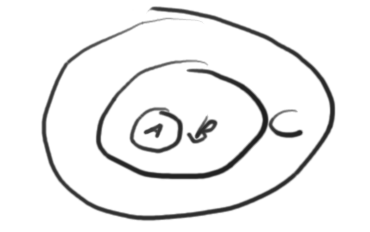
\includegraphics{venn/1}

16. \textit{Use a Venn diagram to illustrate the relationship $A\subset B$
and $A\subset C$.}

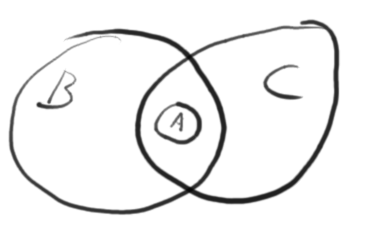
\includegraphics{venn/2}

23A. \textit{How many elements does $\left\{ a,b\left\{ a,b\right\} \right\} $
have?}

3.

23B. \textit{How many elements does $\left\{ \emptyset,a,\left\{ a\right\} ,\left\{ \left\{ a\right\} \right\} \right\} $
have?}

4

23C. \textit{How many elements does $\emptyset$ have?}

0.

27A. $\left\{ a,b,c,d\right\} \times\left\{ y,z\right\} $

$\left(a,y\right),\left(a,z\right),\left(b,y\right),\left(b,z\right),\left(c,y\right),\left(c,z\right),\left(d,y\right),\left(d,z\right)$

27B. $\left\{ y,z\right\} \times\left\{ a,b,c,d\right\} $

$\left(y,a\right),\left(y,b\right),\left(y,c\right),\left(y,d\right),\left(z,a\right),\left(z,b\right),\left(z,c\right),\left(z,d\right)$

33A. $\left\{ 0,1,3\right\} ^{2}$

$\left(0,0\right),\left(0,1\right),\left(0,3\right),\left(1,0\right),\left(1,1\right),\left(1,3\right),\left(3,0\right),\left(3,1\right),\left(3,3\right)$

33B. $\left\{ 1,2,a,b\right\} ^{2}$

$\left(1,1\right),\left(1,2\right),\left(1,a\right),\left(1,b\right),\left(2,1\right),\left(2,2\right),\left(2,a\right),\left(2,b\right)\left(a,1\right),\left(a,2\right),\left(a,a\right),\left(a,b\right),\left(b,1\right),\left(b,2\right),\left(b,a\right),\left(b,b\right)$

34A. $\left\{ a\right\} ^{3}$

$\left(a,a,a\right)$

34B. $\left\{ 0,a\right\} ^{3}$

$\left(0,a\right),\left(a,0\right)$

36. \textit{How many different elements does $A\times B\times C$
have if $A$ has $m$ elements, $B$ has $n$ elements, and $C$ has
$p$ elements?}

$nmp$ elements.

42A. \textit{Translate $\exists x\in R\left(x^{3}=-1\right)$ and
determine its truth value.}

``There exists a real number that, when cubed, is -1.'' True, the
number is -1.

42B. $\exists x\in Z\left(x+1>x\right)$

``There exists an integer that grows when 1 is added.'' True for
all numbers.

42C. $\forall x\in Z\left(x-1\in Z\right)$

``All integers are still integers when 1 is subtracted.'' True.

42D. $\forall x\in Z\left(x^{2}\in Z\right)$

``All integers are still integers when squared.'' True.

44A. \textit{Find the truth set of all integers that satisfy $x^{3}\geq1$.}

All integers greater than 1.

44B. $x^{2}=2$

No integer values.

44C. $x<x^{2}$

All integers, excluding -1, 0 and 1.
\end{document}
